\documentclass[a4paper]{article}

%use the english line for english reports
%usepackage[english]{babel}
\usepackage[portuguese]{babel}
\usepackage[utf8]{inputenc}
\usepackage{indentfirst}
\usepackage{graphicx}
\usepackage{verbatim}


\begin{document}

\setlength{\textwidth}{16cm}
\setlength{\textheight}{22cm}

\title{\Huge\textbf{Jogo de Tabuleiro - Campo Bello}\linebreak\linebreak\linebreak
\Large\textbf{Relatório Final}\linebreak\linebreak
\linebreak\linebreak

\includegraphics[scale=0.1]{feup-logo.png}\linebreak\linebreak
\linebreak\linebreak
\Large{Mestrado Integrado em Engenharia Informática e Computação} \linebreak\linebreak
\Large{Programação em Lógica}\linebreak
}

\author{\textbf{Grupo 04:}\\ João Nuno Fonseca Seixas - 201505648 \\ Renato Alexandre Sousa Campos - 201504942 \\\linebreak\linebreak \\
 \\ Faculdade de Engenharia da Universidade do Porto \\ Rua Roberto Frias, s\/n, 4200-465 Porto, Portugal \linebreak\linebreak\linebreak
\linebreak\linebreak\vspace{1cm}}
%\date{Junho de 2007}
\maketitle
\thispagestyle{empty}

%************************************************************************************************
%************************************************************************************************

\newpage

\section*{Resumo}
	Na unidade curricular de Programação Lógica fomos desafiados a desenvolver um programa, usando a linguagem PROLOG, para simular o jogo de tabuleiro Campo Bello.  

	O maior desafio deste projeto foi desenvolver o jogo usando uma linguagem funcional cujo paradigma é bastante diferente daquele a que estamos habituados a utilizar.

	Outro desafio foi definir e implementar a estrutura de dados, uma vez que uma lista de listas não era muito viável devido ao formato do tabuleiro (triângulos). Neste caso, optamos por representar o tabuleiro como uma espécie de grafo não dirigido, cujas arestas representam saltos válidos e os nós representam posições do tabuleiro.

	Para resolver este problema foram usados predicados já existentes na linguagem, como por exemplo: ! (cut),  member e findall; assim como predicados criados pelo grupo. A maior parte dos predicados criados pelo grupo usam algoritmos recursivos, o que implica criar geralmente 3 predicados: caso base, passo recursivo e outro predicado para gerir erros encontrados no passo recursivo.

	Sumariando, o projeto desenvolvido permitiu aprofundar os nossos conhecimentos práticos de PROLOG e teóricos sobre o paradigma funcional.

\newpage

\tableofcontents

%************************************************************************************************
%************************************************************************************************

%*************************************************************************************************
%************************************************************************************************

\newpage

%%%%%%%%%%%%%%%%%%%%%%%%%%
\section{Introdução}

O objetivo deste trabalho é implementar, em linguagem Prolog, um jogo de tabuleiro para dois jogadores e uma aplicação, em Prolog, para o jogar. O jogo permite jogar em três modos de utilização: Humano/Humano, Humano/Computador e Computador/Computador, e tem dois níveis de jogo para o Computador. 

O relatório segue a seguinte estrutura: O Jogo Campo Bello, onde está descrito a história e principais regras de jogo; Lógica do Jogo, descrição do projeto e a implementação da lógica do jogo em Prolog; Interface com Utilizador, como é feita a interação Utilizador-Programa; Conclusões, principais conclusões e possíveis melhorias do trabalho desenvolvido.


%%%%%%%%%%%%%%%%%%%%%%%%%%
\section{O Jogo Campo Bello}

Campo Bello é um jogo que pode ser jogado de 2 a 4 jogadores. Tem inspiração no jogo clássico "Resta Um" ou "Peg Solitaire" em Inglês. É um jogo ainda recente, criado em 2017.  

Para ganhar, um jogador deve tentar remover todas as suas peças do tabuleiro antes dos adversários.
O tabuleiro consiste em 4 triângulos que rodeiam um diamante central. Os triângulos correspodem às áreas iniciais de cada jogador. As peças são removidas ao saltar:  saltar uma peça nossa causa a remoção da peça que foi saltada; saltar uma peça adversária permite-nos remover uma peça nossa do tabuleiro. 

Na variante de apenas 2 jogadores, que vai ser implementada, os jogadores ficam com triângulos opostos e jogam alternadamente.
É também possível executar saltos duplos e triplos numa só jogada.
No fim do jogo cada jogador pontua 1 ponto por cada uma das suas peças fora da área inicial e 3 pontos por cada uma das suas peças dentro da sua área inicial.
O jogador com menos pontos ganha!\linebreak\linebreak 
\begin{center}
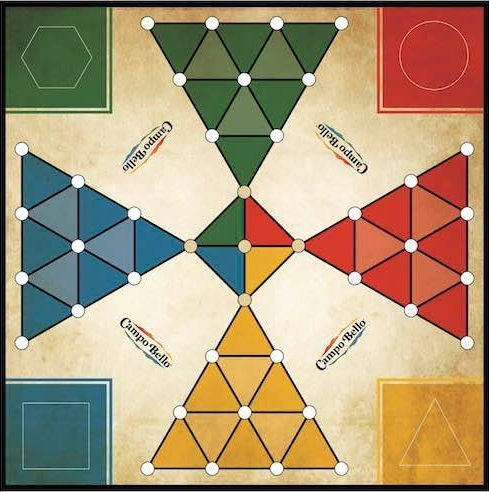
\includegraphics[scale=0.6]{originalBoard.png}\linebreak\linebreak
\end{center}
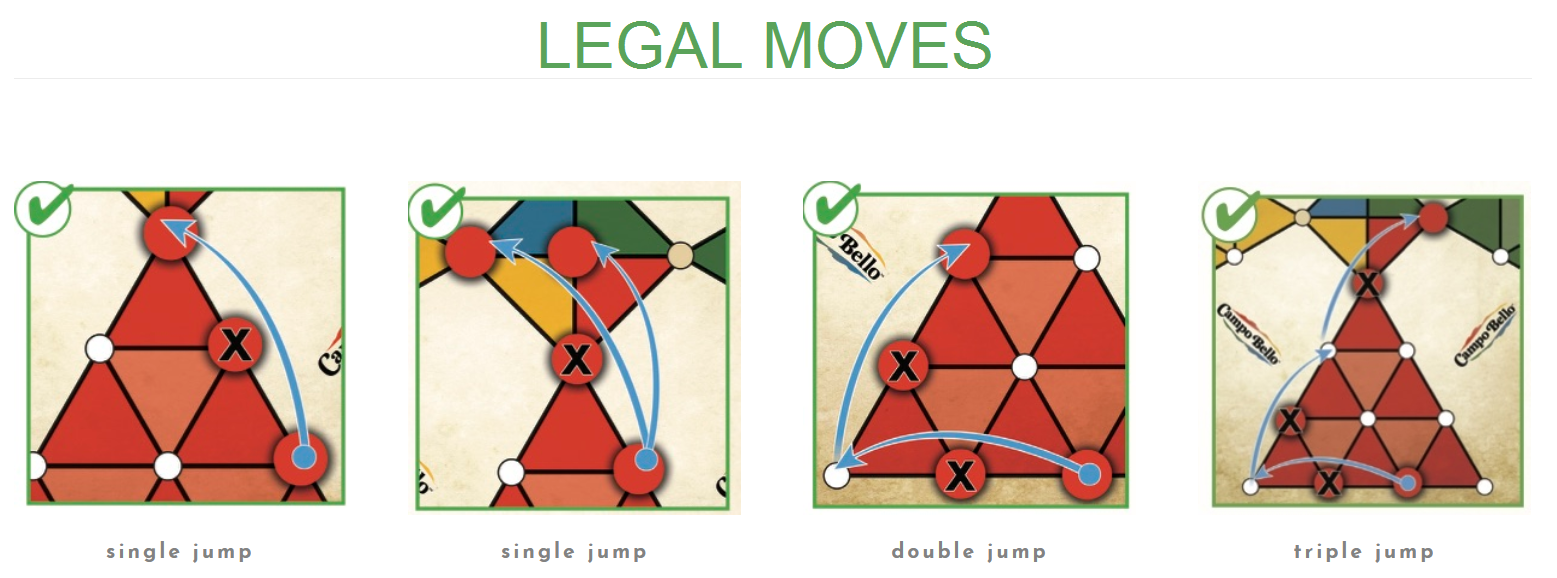
\includegraphics[scale=0.3]{legalMoves.PNG}\linebreak\linebreak
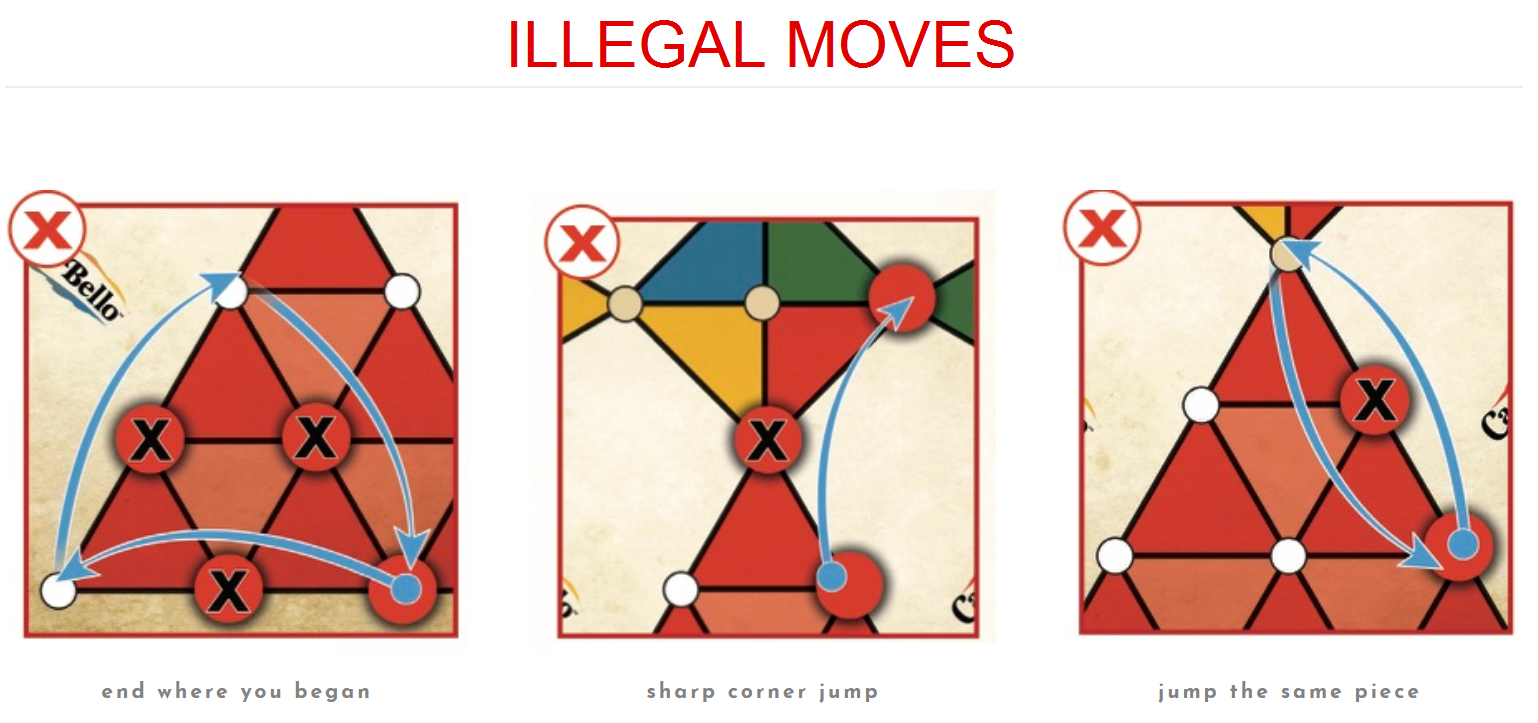
\includegraphics[scale=0.3]{illegalMoves.PNG}\linebreak\linebreak

http://www.campobellogame.com/


%%%%%%%%%%%%%%%%%%%%%%%%%%
\section{Lógica do Jogo}

\subsection{Representação do Estado do Jogo} O estado do jogo é representado por 2 listas que identificam em que posições do tabuleiro estão as peças de cada jogador (1 lista para cada jogador). As peças de cada jogador sáo designadas em Inglês por "movers".\linebreak
\begin{flushleft} 
Tabuleiro no estado de jogo inicial:
\end{flushleft}
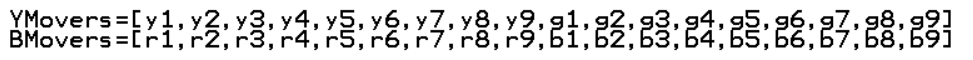
\includegraphics[scale=0.6]{initialBoard.png}\linebreak\linebreak
\begin{flushleft} 
Tabuleiro no estado de jogo intermédio:
\end{flushleft}
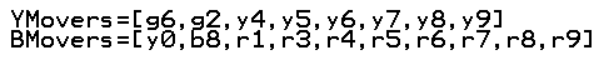
\includegraphics[scale=0.6]{midBoard.png}\linebreak\linebreak
\linebreak
\begin{flushleft} 
Tabuleiro no estado de jogo final:
\end{flushleft}
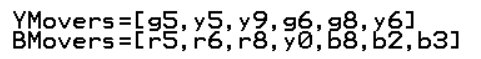
\includegraphics[scale=0.6]{finalBoard.png}\linebreak\linebreak 
Com o decorrer do jogo as listas perdem elementos. O estado final do jogo é alcançado quando uma das listas estiver vazia ou quando não houver mais jogadas possíveis para o jogador que vai jogar.


\subsection{Visualização do Tabuleiro} O predicado para visualização do tabuleiro mostra as posições do tabuleiro do lado esquerdo a usar para os movimentos e do lado direito o estado atual das peças.  Usa \textit{put\_code} para melhorar o aspeto e facilitar a visualização. 

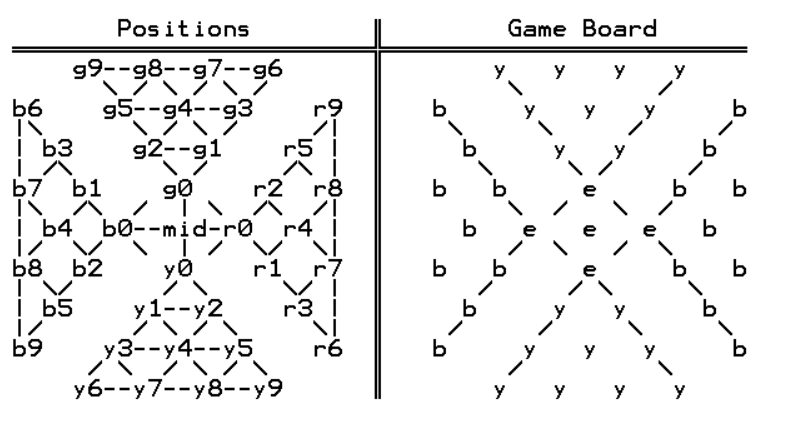
\includegraphics[scale=0.6]{gameBoard.png}\linebreak\linebreak
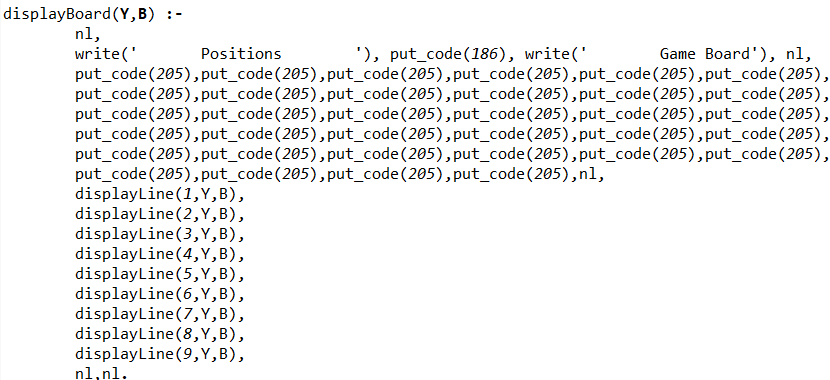
\includegraphics[scale=0.6]{displayBoard.png}\linebreak\linebreak

Estes predicados encarregam-se de imprimir qual a peça do tabuleiro está naquela posição. 

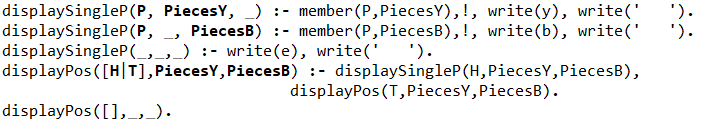
\includegraphics[scale=0.8]{displayBoard1.png}\linebreak\linebreak

O resto é específico de cada linha. Eis o exemplo de uma dessas linhas: 

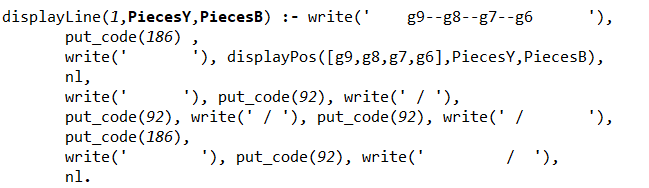
\includegraphics[scale=0.8]{displayBoard2.png}\linebreak\linebreak

\subsection{Lista de Jogadas Válidas} Na implementação do nosso jogo fizemos predicados para definir quais os saltos de peças possiveis, por exemplo estes:

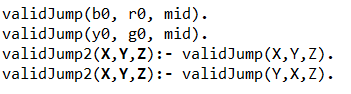
\includegraphics[scale=0.8]{predicados.png}\linebreak\linebreak

Implementamos também os seguintes predicados para obter a lista de todas as jogadas possiveis para qualquer dos jogadores ou para qualquer posição inicial, em que verifica se uma jogada é válida e adiciona-a à lista \textit{Moves}.
\begin{center}
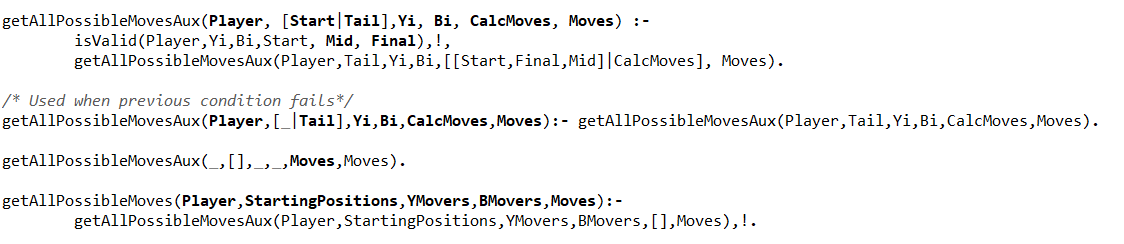
\includegraphics[scale=0.7]{allpossiblemoves.png}\linebreak
\end{center} 
Para uma jogada ser válida vê se cumpre as regras do jogo (ver 3.4).

\subsection{Execução de Jogadas} Valida uma jogada através dos predicados seguintes: 

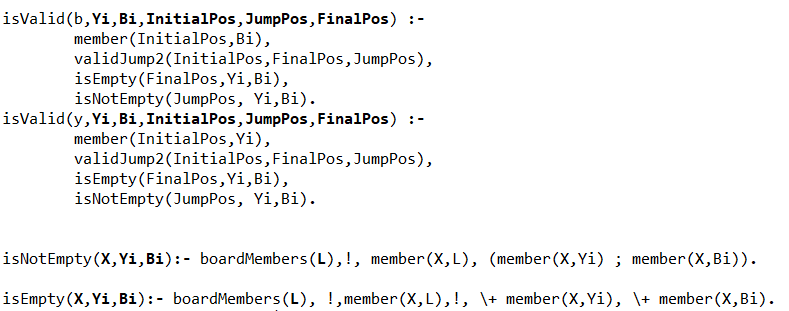
\includegraphics[scale=0.8]{isvalid.png}\linebreak\linebreak 
Só depois executa o predicado \textit{move(+MoverPosY, +MoversPosB, +InitialPos, +JumpPos, +FinalPos, -NewMoversPosY, -NewMoversPosB, +TypeofPlayer)}, em que  \textit{TypeofPlayer} pode ser \textit{human} ou \textit{bot}, em que elimina a peça da posição onde estava e insere na sua nova posição e eliminando a peça que saltou ou eliminando outra das suas peças dependo se a peça que saltou era sua ou se era do adversário. Uma parte deste predicado:

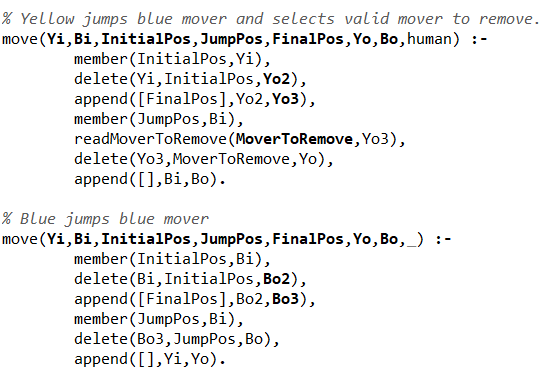
\includegraphics[scale=0.8]{move.png}\linebreak\linebreak 

O nível médio do \textit{bot}, assim como qualquer jogador podem ainda fazer até três saltos consecutivos através dos seguintes predicados: 

\textit{makeConsecutivePlay( +Player, +MoverPosY, +MoversPosB, +FirstInitial, +PrevFinal, -NewMoversPosY, -NewMoversPosB, +TypeofPlayer, +Count)} 

\textit{readConsecutiveMove( +Player, +MoverPosY, +MoversPosB, +FirstInitial, +PrevFinal, +Jump, -Final)} 

E também \textit{getConsecutiveMoveForBot} (ver 3.7).

\subsection{Avaliação do Tabuleiro} No jogo, através do predicado \textit{points}(ver 3.6) que vê quantos pontos um jogador tem, podemos ver se uma jogada é melhor que outra comparando os pontos dos diferentes tabuleiros.

\subsection{Final do Jogo} Verificação do fim do jogo, com identificação do vencedor.
O jogo acaba quando o jogador que vai jogar se encontra sem jogadas possíveis.
\linebreak
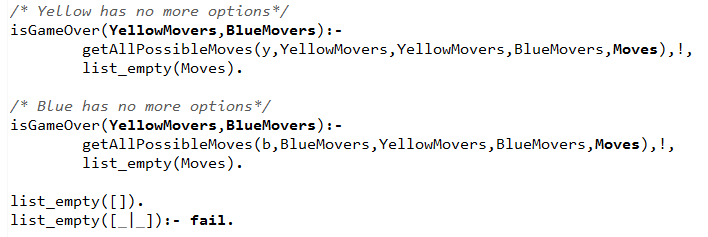
\includegraphics[scale=0.8]{isGameOver1.png}\linebreak\linebreak
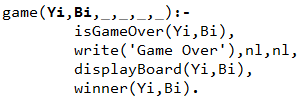
\includegraphics[scale=0.8]{isGameOver2.png}\linebreak\linebreak
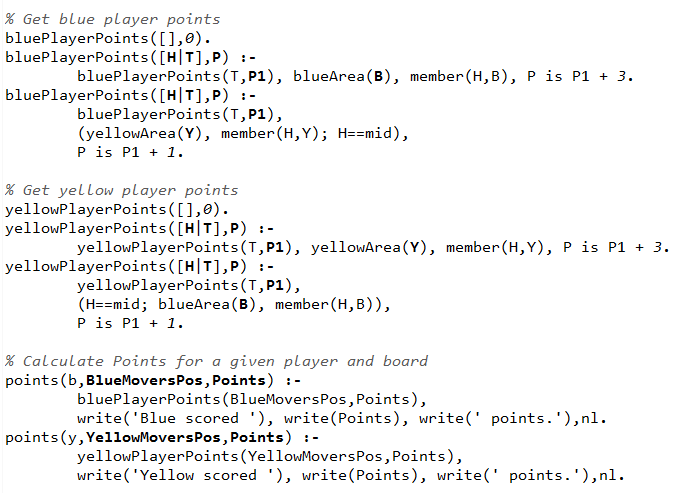
\includegraphics[scale=0.8]{isGameOver3.png}\linebreak\linebreak

\subsection{Jogada do Computador} Escolha da jogada a efetuar pelo computador, dependendo do nível de dificuldade.
Quando o nível de dificulade é 1 o computador apenas faz saltos simples e escolhe sempre o primeiro salto da sua lista de jogadas possíveis.\linebreak
Quando o nível de dificuldade é 2 o computador consegue fazer saltos simples, duplos e triplos, escolhendo sempre a primeira jogada da sua lista de jogadas possíveis.\linebreak
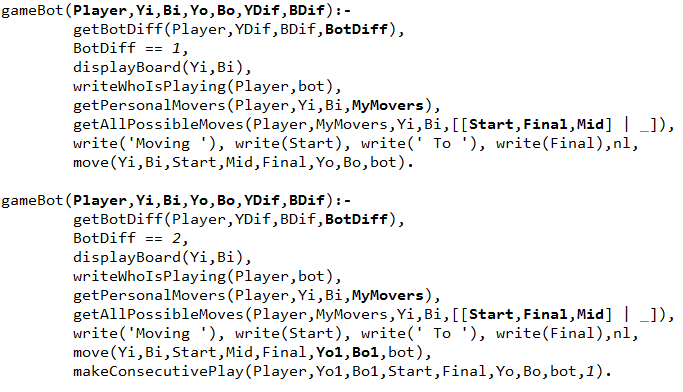
\includegraphics[scale=0.8]{gameBot.png}\linebreak\linebreak



%%%%%%%%%%%%%%%%%%%%%%%%%%
\section{Interface com o Utilizador}
Sempre que existe interação entre o programa e o utilizador, o programa questiona o utilizador até que este introduza uma opção válida.
\begin{flushleft} 
Menu inicial: 
\end{flushleft} 
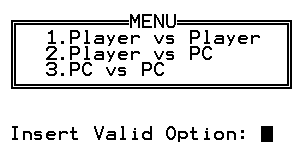
\includegraphics[scale=0.8]{initialMenu.png}\linebreak
\begin{flushleft} 
Caso a opção 2 ou 3 seja escolhida, o programa irá perguntar qual o nível de dificuldade para cada bot.\linebreak
\end{flushleft} 
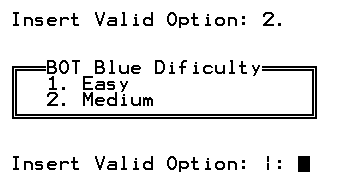
\includegraphics[scale=0.8]{chooseBotDifficulty.png}\linebreak\linebreak
\begin{flushleft} 
Exemplo de interação com o utiizador num salto duplo:\linebreak
\end{flushleft} 
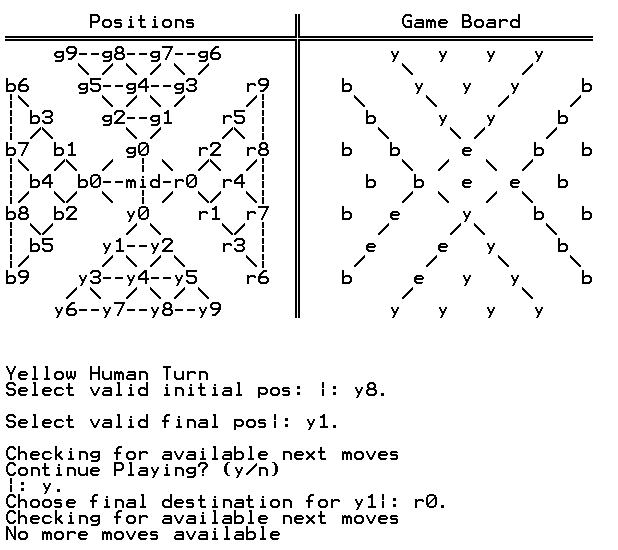
\includegraphics[scale=0.6]{doubleJump.png}\linebreak\linebreak


%%%%%%%%%%%%%%%%%%%%%%%%%%
\section{Conclusões}
Prolog é uma linguagem com grande potencial e é preciso experiência para saber usá-la da melhor forma. É muito fácil escrever código repetitivo e não optimizado.
Para melhorar o trabalho desenvolvido poderiamos melhorar a aleatoriedade das jogadas do bot de nível 1. Em relação ao bot de nível 2 poderíamos ter percorrido a sua árvore de jogadas possíveis, gerar um tabuleiro para cada jogada diferente e de seguida obter o melhor tabuleiro, aquele com menor pontuação, usando o predicado \textit{points(+Player, +PlayerMovers, -Points)}  já criado e demonstrado na secção 3.6.


\clearpage
\addcontentsline{toc}{section}{Bibliografia}
\renewcommand\refname{Bibliografia}
\bibliographystyle{plain}
\bibliography{myrefs}


\end{document}
